% Figure F1_correctness_before_after of study_analysis_001 - generated by thesis/study_analysis/figures.py; do not edit by hand.
% Preamble: \usepackage{pgfplots}
%           \pgfplotsset{compat=1.18}
% Correctness before and after repair (Q06, BASE vs FINAL)
% Caption: figures/F1_correctness_before_after.caption.tex (figure_caption_tex)
% Q06 correctness pass on BASE vs FINAL[v] (identical base-cell cohort, checked) per block
% error bars: 95% CI: nonparametric cluster bootstrap, percentile intervals, stratified by block (pilot benchmarks resampled among the 12 pilot benchmarks, full_ext among its 48); seed 20261017; cluster = benchmark; 2,000 replicates (descriptive, unadjusted)
% BL01: Includes dense_la/00 (BL-01 tolerance convention: possible false FAIL verdicts; disclosure-bearing aggregate); sensitivity SA1 in T10.
% IC1: Q06 is in-sample for test_feedback and combined_feedback: their loops see the ParEval test verdict and stop when it passes (every stopped_tests_pass trajectory is a Q06 pass), so they optimise the endpoint; for static_feedback Q06 is out-of-sample (measured once in phase 2, never seen by the loop). The variants therefore differ in trigger and stop rules, not only in feedback content; test_feedback cannot regress on Q06 by construction.
% IC6: static_feedback repair triggers are dominated by clang-tidy bugprone findings and, on MPI, by low-confidence hints (design document: no trustworthy static MPI tool exists); static_feedback results measure this frozen blocking-set configuration, not static analysis in general.
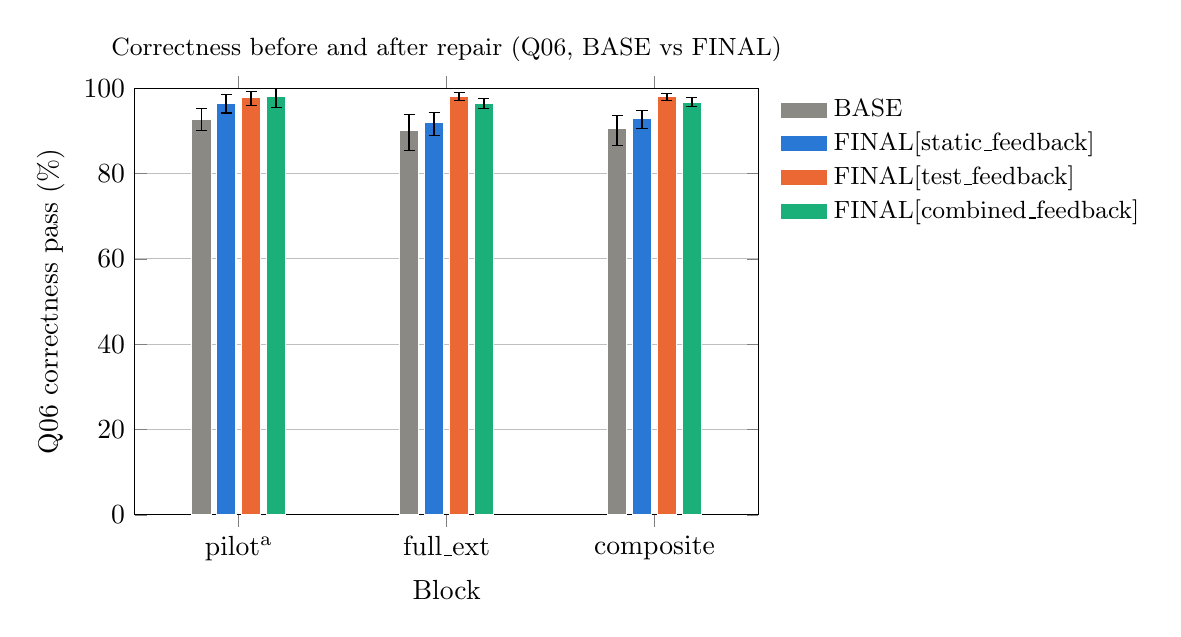
\begin{tikzpicture}
\definecolor{saSeriesA}{HTML}{8A8984}
\definecolor{saSeriesB}{HTML}{2A78D6}
\definecolor{saSeriesC}{HTML}{EB6834}
\definecolor{saSeriesD}{HTML}{1BAF7A}
\begin{axis}[
  width=9.5cm,
  height=7cm,
  ybar,
  bar width=7.000pt,
  enlarge x limits=0.25,
  ymin=0.000,
  ymax=100.000,
  xtick={0,1,2},
  xticklabels={{pilot\textsuperscript{a}},{full\_ext},{composite}},
  xlabel={Block},
  ylabel={Q06 correctness pass (\%)},
  ymajorgrids,
  legend cell align=left,
  legend style={at={(1.02,1)},anchor=north west,font=\small,draw=none},
  title={Correctness before and after repair (Q06, BASE vs FINAL)},
  title style={font=\small}
]
\addplot[draw=white, fill=saSeriesA, area legend, bar shift=-13.500pt] coordinates {(0,92.677) (1,90.088) (2,90.606)};
\addlegendentry{BASE}
\addplot[forget plot, draw=none, fill=none, bar shift=-13.500pt, error bars/.cd, y dir=both, y explicit, error bar style={draw=black, line width=0.6pt}] coordinates {(0,92.677) += (0,2.525) -= (0,2.525) (1,90.088) += (0,3.725) -= (0,4.735) (2,90.606) += (0,2.981) -= (0,3.941)};
\addplot[draw=white, fill=saSeriesB, area legend, bar shift=-4.500pt] coordinates {(0,96.465) (1,91.919) (2,92.828)};
\addlegendentry{FINAL[static\_feedback]}
\addplot[forget plot, draw=none, fill=none, bar shift=-4.500pt, error bars/.cd, y dir=both, y explicit, error bar style={draw=black, line width=0.6pt}] coordinates {(0,96.465) += (0,2.020) -= (0,2.273) (1,91.919) += (0,2.399) -= (0,2.967) (2,92.828) += (0,1.970) -= (0,2.374)};
\addplot[draw=white, fill=saSeriesC, area legend, bar shift=4.500pt] coordinates {(0,97.727) (1,98.106) (2,98.030)};
\addlegendentry{FINAL[test\_feedback]}
\addplot[forget plot, draw=none, fill=none, bar shift=4.500pt, error bars/.cd, y dir=both, y explicit, error bar style={draw=black, line width=0.6pt}] coordinates {(0,97.727) += (0,1.515) -= (0,1.768) (1,98.106) += (0,0.884) -= (0,1.010) (2,98.030) += (0,0.758) -= (0,0.859)};
\addplot[draw=white, fill=saSeriesD, area legend, bar shift=13.500pt] coordinates {(0,97.980) (1,96.465) (2,96.768)};
\addlegendentry{FINAL[combined\_feedback]}
\addplot[forget plot, draw=none, fill=none, bar shift=13.500pt, error bars/.cd, y dir=both, y explicit, error bar style={draw=black, line width=0.6pt}] coordinates {(0,97.980) += (0,2.020) -= (0,2.525) (1,96.465) += (0,1.073) -= (0,1.201) (2,96.768) += (0,0.960) -= (0,1.010)};
\end{axis}
\end{tikzpicture}
